\documentclass{report}

\author{ImJaviPerez}
\usepackage{tikz}
%\usetikzlibrary{shapes,arrows,positioning}
\usetikzlibrary{automata,arrows,positioning,calc}


\begin{document}
Markov chain:	
\begin{center}
	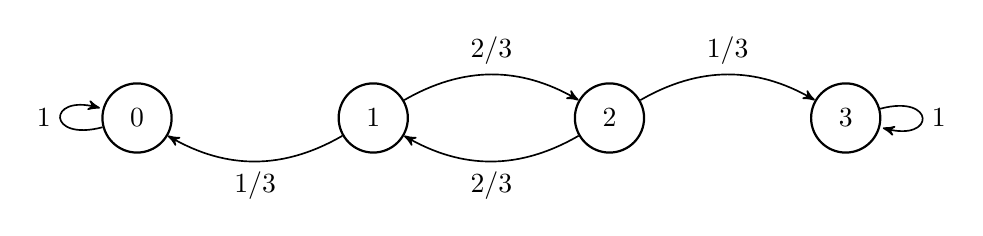
\begin{tikzpicture}[->, >=stealth', auto, semithick, node distance=3cm]
	\tikzstyle{every state}=[fill=white,draw=black,thick,text=black,scale=1]
	\node[state]    (A)                     {$0$};
	\node[state]    (B)[right of=A]   {$1$};
	\node[state]    (C)[right of=B]   {$2$};
	\node[state]    (D)[right of=C]   {$3$};
	\path
	(A) edge[loop left]			node{$1$}	(A)
	(B) edge[bend left,below]	node{$1/3$}	(A)
	edge[bend left,above]		node{$2/3$}	(C)
	(C) edge[bend left,below]	node{$2/3$}	(B)
	edge[bend left,above]		node{$1/3$}	(D)
	(D) edge[loop right]		node{$1$}	(D);
	%\node[above=0.5cm] (A){Patch G};
	%\draw[red] ($(D)+(-1.5,0)$) ellipse (2cm and 3.5cm)node[yshift=3cm]{Patch H};
	\end{tikzpicture}
\end{center}
	
\end{document}